\documentclass[a4paper,10pt]{ctexart} %ctexart
\usepackage[backref,hidelinks]{hyperref} %hidelinks去掉引用处的红框
\pagestyle{plain} %把页码从右上角移到页脚
%==========打印代码的设置===================
\usepackage{color}
\definecolor{gray}{rgb}{0.8,0.8,0.8}
\usepackage{listings}
\lstset{basicstyle=\small}
\lstset{numbers=left} \lstset{language=C++} \lstset{breaklines}
\lstset{extendedchars=false} \lstset{backgroundcolor=\color{gray}}
\lstset{keywordstyle=\color{blue}\bfseries} \lstset{frame=none}
\lstset{tabsize=4} \lstset{commentstyle=\color{red}}
\lstset{stringstyle=\emph}
%=======================================
\begin{document}
\begin{center}
\textbf{AP\_InertialNav.cpp}
\end{center}

惯导系统通过积分加速度计的读数来获得速度与位置信息,随时间增长会产生积累误差。InertialNav中的函数用于修正速度和位置。加速度-速度-位置构成三阶系统,通过将位置误差\_position\_error积分后反馈到各物理量,形成三个反馈回路,实现闭环控制。

主要函数为update(),check\_gps()和check\_baro(),整体结构如图所示,虚线左侧由update()实现,虚线右侧由check\_gps()和check\_baro()实现:
\begin{figure}[!htb]\centering
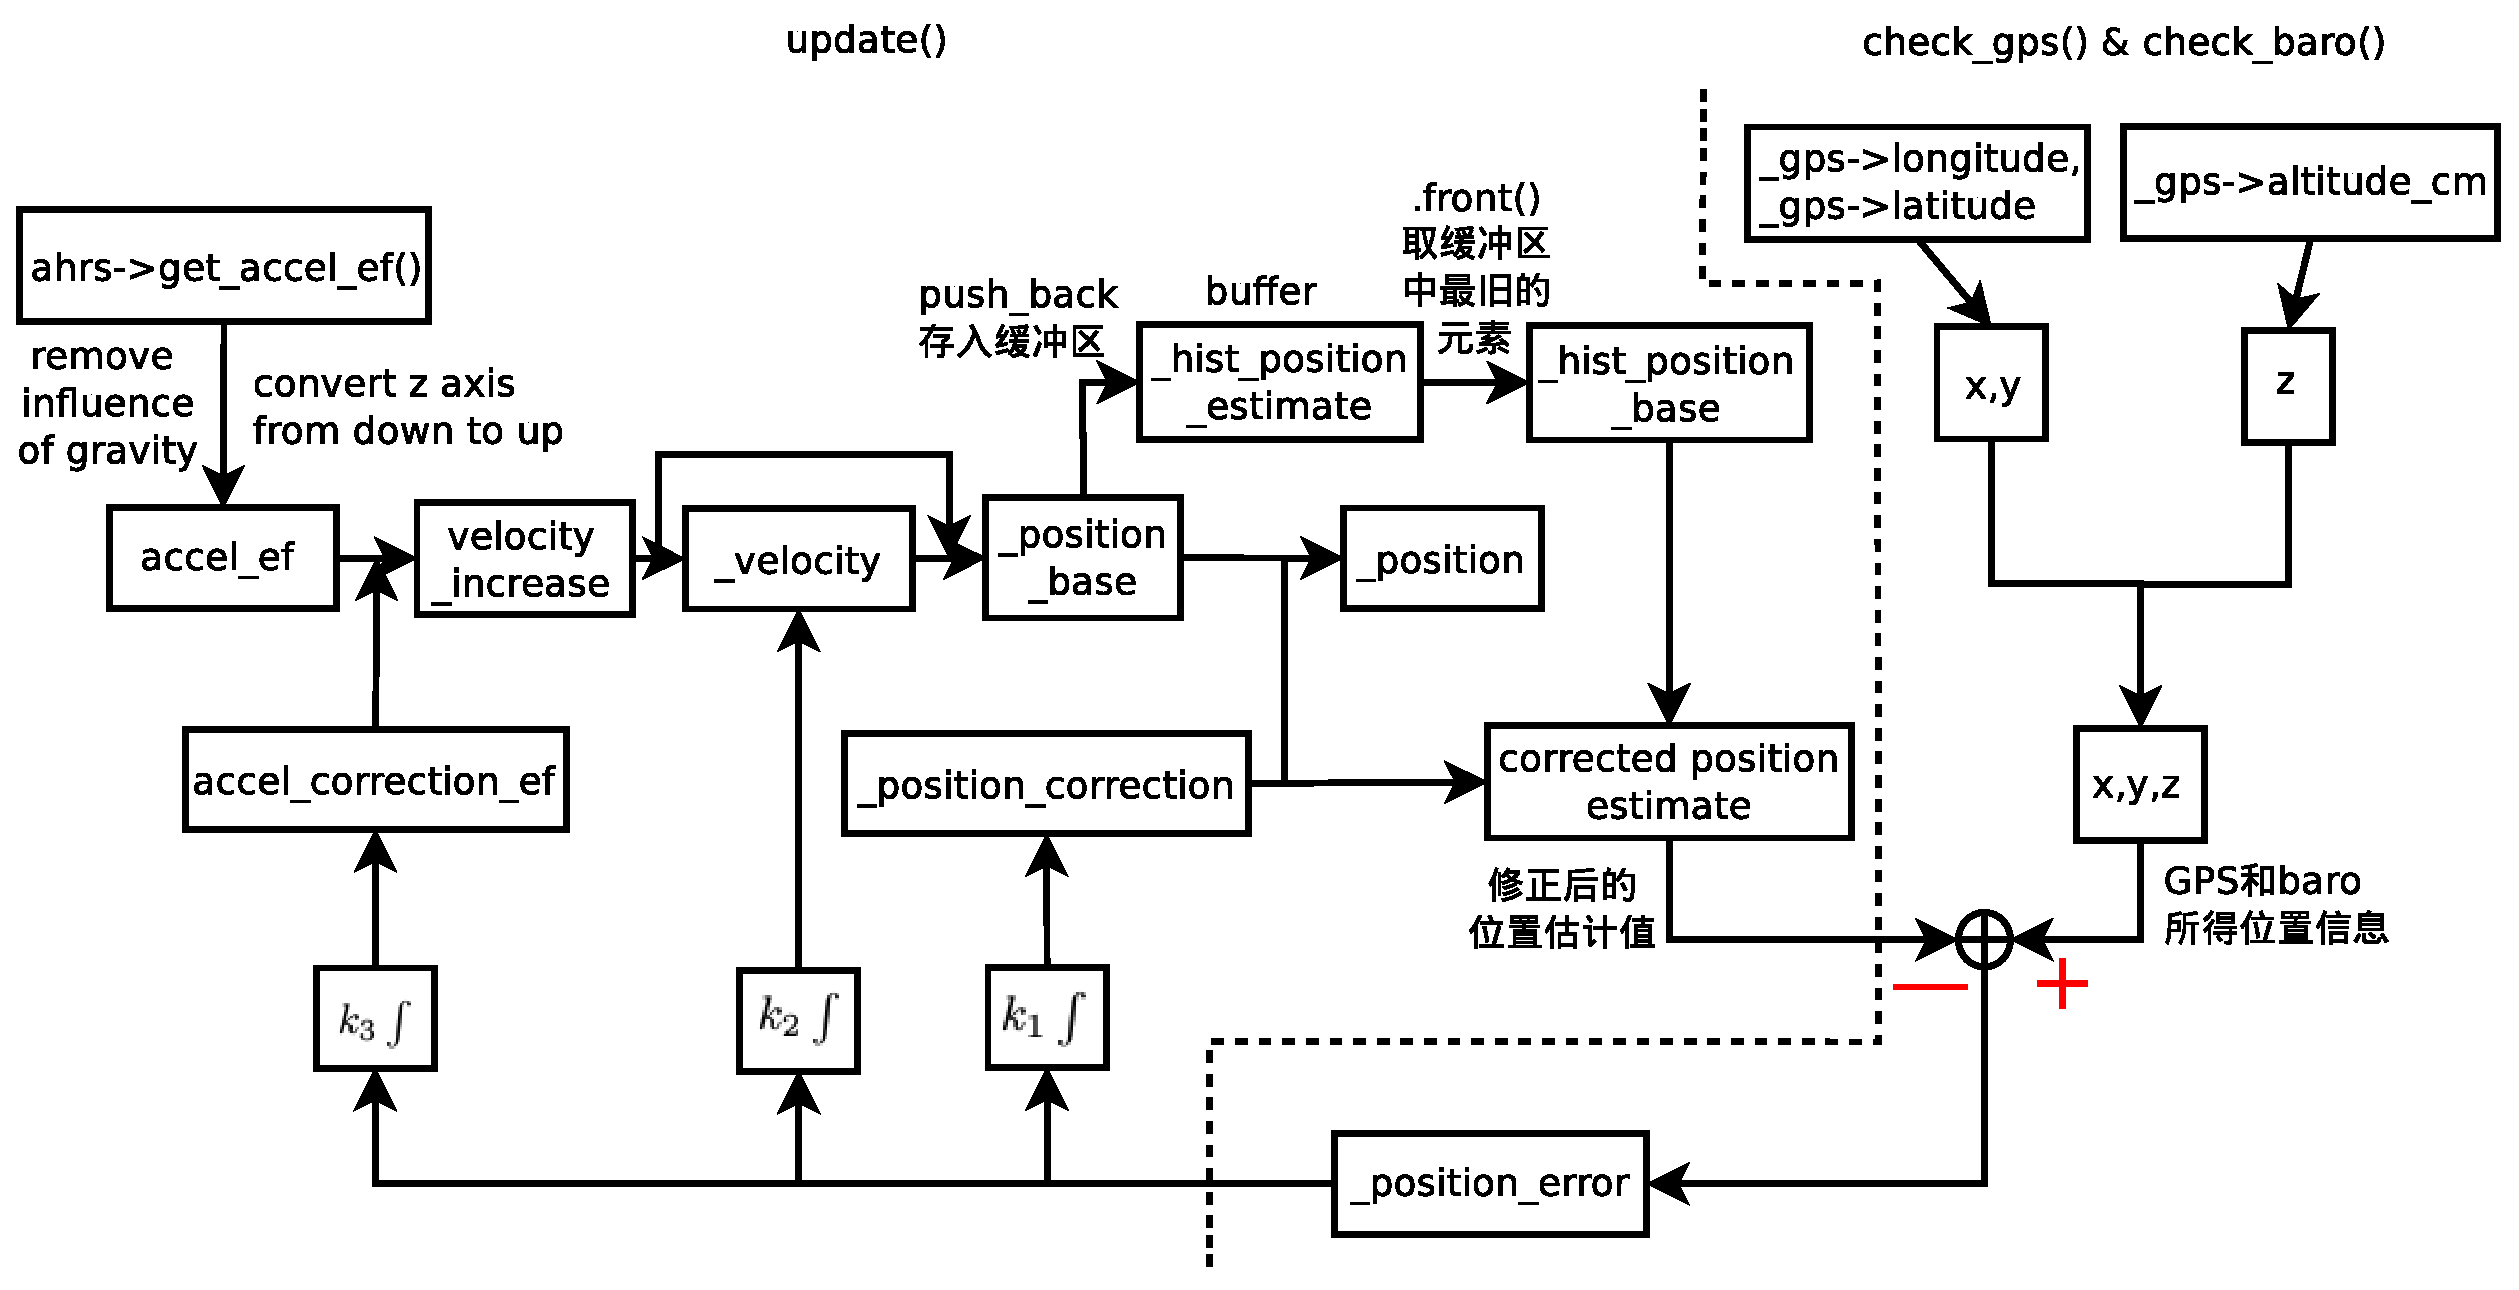
\includegraphics[scale=0.3]{InertialNav_update.eps}
\caption{InertialNav}\label{fig:InertialNav_update} %scale=0.4
\end{figure}


\noindent 修正具体分为两个通道:\\
1.horizontal:使用GPS信息修正水平位置;\\
2.vertical:\phantom{tal}使用Barometer信息修正高度。

\vspace{10pt}
\noindent 主要步骤:

\noindent 1.init()

初始化。调用update\_gains()函数,使用互补滤波时间常数计算控制增益\_k1\_xy,\_k2\_xy,\_k3\_xy和\_k1\_z,\_k2\_z,\_k3\_z。
\begin{lstlisting}
        _k1_xy = 3 / _time_constant_xy;
        _k2_xy = 3 / (_time_constant_xy*_time_constant_xy);
        _k3_xy = 1 / (_time_constant_xy*_time_constant_xy*_time_constant_xy);
        
        _k1_z = 3 / _time_constant_z;
        _k2_z = 3 / (_time_constant_z*_time_constant_z);
        _k3_z = 1 / (_time_constant_z*_time_constant_z*_time_constant_z);
\end{lstlisting}

从增益的形式来看,系统采用了扩张状态观测器。GPS和baro所得位置信息与修正后的位置估计值的差值(即\_position\_error)为观测误差,增益为\_k3的状态变量(即accel\_correction\_ef)是扩张变量。
状态观测器的特征多项式为:
\begin{equation}
\lambda^3+3\lambda^2+3\lambda+1=(\lambda+1)^3
\end{equation}
其满足 Hurwitz 条件,故能够保证观测误差的快速收敛。
从而,通过状态反馈(将accel\_correction\_ef补偿到accel\_ef),实现了对位置和速度的修正。

\vspace{10pt}
\noindent 2.update(float dt)

如果GPS和气压计有新数据可用,使用最新信息更新速度和位置。

\noindent 函数调用关系:\\
\vspace{-20pt}
%\begin{table}[!htb]
\begin{tabular}{lll}
update()->  & check\_baro()		&	\\
			& check\_gps()->	& correct\_with\_gps()	\\
			&					& correct\_with\_baro()
\end{tabular}
%\end{table}

\vspace{20pt}
\noindent correct\_with\_gps()和correct\_with\_baro()用于计算\_position\_error。注意到代码中传递给check\_gps()调用的correct\_with\_baro()的参数是\_gps->altitude\_cm-\_home\_alt,而check\_baro()调用correct\_with\_baro()的语句被if(0)跳过,即实际使用了gps而不是baro来获得高度。update()实现图\ref{fig:InertialNav_update}中的其余部分。

结合流程图分析代码:\\
1) 调用函数check\_baro()和check\_gps()获取位置信息,并计算加速度计所得位置估计值的误差\_position\_error:
\begin{lstlisting}
    // check if new baro readings have arrived and use them to correct vertical accelerometer offsets.
    check_baro();

    // check if new gps readings have arrived and use them to correct position estimates
    check_gps();
\end{lstlisting}
2) 使用ahrs获得加速度计读数,然后进行处理:去除重力加速度的影响,然后修改坐标系定义,将z轴由向下改为向上:
\begin{lstlisting}
    Vector3f accel_ef = _ahrs->get_accel_ef();  ///accelerometer values in the earth frame

    // remove influence of gravity
    accel_ef.z += GRAVITY_MSS;
    accel_ef *= 100;

    //Convert North-East-Down to North-East-Up
    accel_ef.z = -accel_ef.z;
\end{lstlisting}
3) 建立反馈回路,将位置误差\_position\_error乘以相应的系数反馈到加速度、速度和位置中:
\begin{lstlisting}
    float tmp = _k3_xy * dt;
    accel_correction_ef.x += _position_error.x * tmp;
    accel_correction_ef.y += _position_error.y * tmp;
    accel_correction_ef.z += _position_error.z * _k3_z  * dt;

    tmp = _k2_xy * dt;
    _velocity.x += _position_error.x * tmp;
    _velocity.y += _position_error.y * tmp;
    _velocity.z += _position_error.z * _k2_z  * dt;

    tmp = _k1_xy * dt;
    _position_correction.x += _position_error.x * tmp;
    _position_correction.y += _position_error.y * tmp;
    _position_correction.z += _position_error.z * _k1_z  * dt;
\end{lstlisting}
\begin{eqnarray}
a_{correction\_ef}	  & = & \int_{0}^{t}{\varepsilon_{position}}\cdot k_{1}\cdot d\tau \\ \nonumber
v_{correction}		  & = & \int_{0}^{t}{\varepsilon_{position}}\cdot k_{2}\cdot d\tau \\ \nonumber
position_{correction} & = & \int_{0}^{t}{\varepsilon_{position}}\cdot k_{3}\cdot d\tau
\end{eqnarray}
$\varepsilon_{position}$即\_position\_error。$k_1$是反馈到加速度的增益系数,$k_2$是反馈到速度的增益系数,$k_3$是反馈到位置的增益系数。注意每个回路的水平通道增益(k\_xy)和高度通道增益(k\_z)不同。

4) 将时间间隔dt内的运动视为匀加速运动,计算速度增量velocity\_increase,更新(未修正的)位置估计值\_position\_base和速度\_velocity:
\begin{lstlisting}
    // calculate velocity increase adding new acceleration from accelerometers
    const Vector3f &velocity_increase = (accel_ef + accel_correction_ef) * dt;

    // calculate new estimate of position
    _position_base += (_velocity + velocity_increase*0.5) * dt;

    // update the corrected position estimate
    _position = _position_base + _position_correction;

    // calculate new velocity
    _velocity += velocity_increase;
\end{lstlisting}
即
\begin{eqnarray}
\Delta v	&=&	(a_{ef}+a_{correction\_ef})dt\\ \nonumber
\Delta s	&=&	(v+\frac{1}{2}\Delta v)t\\ \nonumber
v			&=&	v+\Delta v
\end{eqnarray}
式中$\Delta v$为velocity\_increase,$\Delta s$为\_position\_base的增量。

5) 将得到的位置估计值存入buffer \_hist\_position\_estimate\_x/y/z。这样做的原因是,由于GPS信息的传输存在延迟,其数据落后于加速度计得到的数据。将加速度计得到的实时数据存入buffer,buffer的容量即延迟时间内的采样数据量,这样,与GPS数据进行比较求位置误差时,使用buffer中最旧的数据即可消除延迟的影响。
\begin{lstlisting}
    // store 3rd order estimate (i.e. estimated vertical position) for future use
    _hist_position_estimate_z.push_back(_position_base.z);  /// push_back: add an item to the end of the buffer.buffer大小:15

    // store 3rd order estimate (i.e. horizontal position) for future use at 10hz
    _historic_xy_counter++;
    if( _historic_xy_counter >= AP_INTERTIALNAV_SAVE_POS_AFTER_ITERATIONS ) {   ///10,函数调用应该是100hz,因此调用10次存一次数据
        _historic_xy_counter = 0;
        _hist_position_estimate_x.push_back(_position_base.x); 	//buffer大小:5
        _hist_position_estimate_y.push_back(_position_base.y);
    }

\end{lstlisting}



\begin{flushright}
\vspace{30pt}
2015.8.4\\
方酉
\end{flushright}

\end{document}